%!TEX root = ../template.tex
%%%%%%%%%%%%%%%%%%%%%%%%%%%%%%%%%%%%%%%%%%%%%%%%%%%%%%%%%%%%%%%%%%%%
%% chapter2.tex
%% NOVA thesis document file
%%
%% Chapter with the template manual
%%%%%%%%%%%%%%%%%%%%%%%%%%%%%%%%%%%%%%%%%%%%%%%%%%%%%%%%%%%%%%%%%%%%

\typeout{NT FILE chapter2.tex}%


\chapter{Background}
\label{cha:Background}

In this chapter we present the necessary background for the formal verification field and the elected tools.

\section{Operational Semantics}
\label{sec:Operational_Semantics}

Operational semantics provide a formal framework to define the behaviour of programming languages by describing 
how programs execute step by step. Unlike denotational semantics, which maps programs to mathematical objects, or 
axiomatic semantics, which focuses on logical reasoning about program correctness, operational semantics are particularly 
well-suited for modelling concrete computation and the dynamics of program execution. A foundational style of 
this approach is Structural Operational Semantics (SOS), introduced by Plotkin~\cite{plotkin_81_structural}, which defines program behaviour 
through a set of syntactic transition rules that describe how individual program constructs evolve during execution.

Operational semantics is often split into two main approaches: small-step (reduction-based) and big-step (natural) semantics. 
The small-step approach breaks down computation into a sequence of individual steps, making it useful for analysing intermediate 
program states, as well as properties like divergence or concurrency. In contrast, big-step semantics describes how entire expressions 
evaluate to final values in one go, which is more straightforward for reasoning about the overall behaviour of a 
program~\cite{abs-0808-0586}. However, big-step semantics had a challenge when it came to handling non-terminating behaviour, so 
Leroy and Grall~\cite{abs-0808-0586} introduced coinductive definitions to model both termination and divergence within a single framework. 
This innovation has played a key role in the development of verified compilers and proof systems like Coq.

In the semantics of modern programming languages, particularly those that integrate both functional and imperative paradigms, such as 
\ocaml and \cml, it becomes necessary to extend traditional operational semantics to accurately capture features like mutable state, 
exceptions and references~\cite{0001MS0U22}.

\section{Hoare logic}
\label{sec:Hoare_logic}

Hoare Logic is a formal system for reasoning about the correctness of computer programs. However, 
computer arithmetic often differs from the standard arithmetic familiar to mathematicians due to issues like finite 
precision, overflows, and machine-specific behaviours. To account for these differences, Hoare introduced a new logic~\cite{Hoare69}
based on assertions and inference rules for reasoning about the partial correctness of programs. Drawing inspiration 
from mathematical axioms and formal proof techniques, he proposed a framework where program behaviour could be specified 
and verified using logical formulas. This laid the foundation for systematic program verification and emphasized the need 
to model computational constraints, such as those arising from the limitations of machine arithmetic, within a formal system.

In Cook's seminal work~\cite{0207005}, Hoare Logic was significantly strengthened, since Cook presented a Hoare-style axiom system 
tailored to a simple programming language and rigorously established both its soundness and adequacy. He concluded that, under 
reasonable assumptions, Hoare Logic is not only intuitively effective but also formally complete as a system for reasoning about 
program correctness.

\subsection{Hoare Triples}

The main construction of Hoare logic is the \textit{Hoare triple}, where $P$ is a pre-condition, $C$ is a program (or a fragment)
and $Q$ is a post-condition:

\[ 
  \{P\}\; C \;\{Q\}
\]

A Hoare triple expresses a partial correctness guarantee: if the pre-condition $P$ holds before executing a program fragment 
$C$, and if $C$ terminates, then the post-condition $Q$ will hold afterward. This is a partial correctness result since the 
termination of $C$ is not assured by the triple. Total correctness is achieved when termination is also guaranteed.

\subsection{Assignment Axiom}

\[ 
  \inferrule
  { \ }
  {\{P_0\} \ \textit{x} := \textit{f} \ \{P\}}
  \quad (assign)
\]

Where $x$ is a variable identifier; $f$ is an expression; $P_0$ is obtained from $P$ by substituting $f$ for all occurrences 
of $x$.

The axiom expresses that to prove a post-condition $P$ holds after assigning the expression $f$ to the variable $x$,
it suffices to prove the pre-condition $P_0$ before the assignment, where $P_0$ is obtained by substituting every occurrence of
$x$ in $P$ with the expression $f$.

\subsection{Rule of Composition}

The inference rule for composition states that if the post-condition of the first program segment matches the pre-condition 
of the second, then the entire program will produce the intended result, assuming the initial pre-condition of the first 
segment holds.

\[ 
  \inferrule
  {P\; \{ Q_1 \} \;R_1 \quad \quad  R_1\; \{ Q_2 \} \;R}
  {P\; \{ (Q_1 ; Q_2) \} \;R} 
  \quad (composition)
\]

\subsection{Weakest Pre-Condition Calculus}

After setting an elegant axiomatic framework for reasoning about program correctness through the use of Hoare triples 
$\{P\}\,C\,\{Q\}$, its practical application in large-scale or automated verification tasks presents significant challenges. 
Chief among these is the burden of manually identifying appropriate pre-conditions and invariants. To address this, 
Dijkstra~\cite{Dijkstra76} introduced the weakest pre-condition calculus, which reformulates program correctness into a computational 
problem: given a command $C$ and a desired post-condition $Q$, the function $wp(C,Q)$ computes the weakest pre-condition $P$ 
such that $\{P\}\,C\,\{Q\}$ holds.

This transformation from proof obligations to a calculable pre-condition function represents a critical step toward automating 
program verification. Unlike Hoare's original formulation, which requires deductive reasoning to derive correctness properties, 
weakest pre-condition semantics allow for algorithmic generation of verification conditions, thereby enabling integration 
with automated theorem provers and SMT solvers. The influence of weakest pre-conditions is particularly evident in modern 
deductive verification tools such as \whythree~\cite{boogie11why3}, and \textsf{Dafny}~\cite{Leino10}.

\section{OCaml}
\label{sec:OCaml}

\ocaml is a statically typed functional programming language rooted in the ML family, originally developed 
to serve as the implementation language for theorem provers such as LCF. It inherits the foundational principles 
of typed $\lambda$-calculus, formal logic, and abstract interpretation, and extends them through practical language design 
aimed at enabling both expressiveness and efficiency~\cite{FilliatrePereiraSousa2018}.

First released in the mid-1990s, \ocaml is the principal evolution of the Caml dialect of the ML family. The name \ocaml, 
originally short for Objective Caml, reflects the addition of object-oriented features to the Caml language. While Caml 
stood for Categorical Abstract Machine Language, \ocaml moved away from its dependence on the original abstract machine 
model~\cite{leroy:inria-00070049}. The language is primarily developed and maintained by INRIA, which continues to guide 
its implementation and evolution.

\ocaml distinguishes itself from many academically inspired languages through its strong emphasis on performance. Its static 
type system eliminates the need for runtime type checking by ensuring type correctness at compile time, thereby avoiding the 
performance overhead commonly associated with dynamically typed languages. This design enables \ocaml to maintain high 
execution efficiency while preserving strong safety guarantees at runtime. Exceptions to this safety model arise only in 
specific low-level scenarios, such as when array bounds checking is explicitly disabled or when employing type-unsafe features 
like runtime serialization~\cite{FilliatrePereiraSousa2018}.

For the standard compiler toolchain features, \ocaml has both a high-performance native-code compiler (\textsf{ocamlopt}) and a 
bytecode compiler (\textsf{ocamlc}). The native-code compiler produces efficient machine code via a sophisticated optimizing 
backend~\cite{abs-1011-1783}, while the bytecode compiler offers portability and rapid development. Both compilers are integrated 
with a runtime system that supports automatic memory management via a garbage collector and provides facilities for exception handling, 
concurrency, and system interaction.

\subsection{Immutability by default}

Immutability is promoted as a default design principle in this language. Rather than modifying existing values, new ones 
are created through expression evaluation. This absence of mutable shared state simplifies reasoning about program behaviour 
and eliminates many common sources of verification complexity, such as aliasing and unintended side effects.

\begin{ocamlenv}
  let x = 5
  let y = x + 1 (* x is not modified, just referenced *)
\end{ocamlenv}

Since values are not modified in place, program semantics are preserved under substitution, facilitating referential transparency, 
making symbolic execution and logical reasoning over programs more straightforward in deductive verification.

\subsection{ADTs (Algebraic Data Types)}
\label{subsec:ADT}

In \ocaml, data types fall into three broad categories: atomic predefined types (e.g., \texttt{int}, \texttt{bool}), type 
constructors provided by the language (e.g., \texttt{list}, \texttt{array}, \texttt{option}), and user-defined types, which 
are declared through the general mechanism of algebraic data types, for instance:

\begin{ocamlenv}
  type 'a tree =
    | Leaf
    | Node of 'a tree * 'a * 'a tree
\end{ocamlenv}

A tree can either be a \inlinecode{Leaf}, which represents the empty tree, or a \inlinecode{Node}, which is a tuple with three elements, 
the subtree to the left, the value for the node and the subtree to the right, respectively.

ADTs support exhaustive pattern matching, which is particularly useful for enabling structural recursion and inductive reasoning.
From a verification perspective, this ensures all possible cases are covered, making formal reasoning both precise and complete.
One example of pattern matching combined with ADTs is:

\begin{ocamlenv}
  let rec cmp t1 t2 =
    match t1, t2 with
    | Leaf, Leaf -> true
    | Leaf, _ -> false
    | _, Leaf -> false
    | Node (l1,x1,r1), Node (l2,x2,r2) -> cmp l1 l2 && x1 = x2 && cmp r1 r2
\end{ocamlenv}

The function \inlinecode{cmp} uses exhaustive pattern matching to compare structurally the two trees. When a tree is a leaf it means it is
empty, as such, two empty trees are always equal. By contrast if one is a leaf, but the other is not, then they are different, since
a node represents a non-empty tree. Finally, if both are nodes then it depends on the respective root and subtrees, in which case we have to 
recursively call the function \inlinecode{cmp} for the right and left subtrees.

\subsection{First-Class and Higher-Order Functions}

\ocaml treats functions as first-class values: they can be passed as arguments, returned from other functions, 
and stored in data structures. Combined with lexical scoping and immutable data, this makes \ocaml particularly 
well-suited for working with higher-order abstractions, a feature that aligns naturally with formal systems based on 
higher-order logic.

\begin{ocamlenv}
  let apply_twice f x = f (f x)
  let square x = x * x
  let result = apply_twice square 2  (* returns 16 *)
\end{ocamlenv}

In the context of deductive verification, such functional abstractions support elegant formulations of parametric specifications 
and reasoning principles.

\subsection{Side Effects in OCaml}
\label{subsec:SideEffects}

\ocaml is not a purely functional language since it allows the use of imperative constructs with side effects, like references,
exceptions, built-in arrays, for and while loops. References allow the manipulation of memory, a feature not common for functional
languages. A simple example about Euclidean division is displayed below:

\begin{ocamlenv}
let rec eudiv_aux x y r q =
  if !r >= y then (r := !r - y; q := !q + 1; eudiv_aux x y r q)
  else ()

let euclidean_div x y =
    let r = ref x and q = ref 0 in 
  eudiv_aux x y r q;
  (!q, !r)
\end{ocamlenv}

The main function \inlinecode{euclidean\_div} receives the two arguments \inlinecode{x} and \inlinecode{y}, which represent respectively
the dividend and divisor. This function initializes the remainder \inlinecode{r} as a reference with the value of the dividend 
\inlinecode{x} and the quotient \inlinecode{q} as a reference of value 0. Since these variables are references, the auxiliary function
may alter their in-memory value and by the end of its execution, the references \inlinecode{q} and \inlinecode{r} point to the correct 
values.

This example has the need for an auxiliary function, \inlinecode{eudiv\_aux}, which receives as arguments the dividend 
\inlinecode{x}, the divisor \inlinecode{y}, the remainder \inlinecode{r}, and the quotient \inlinecode{q}. This function recursively
increments the quotient by 1 and subtracts the remainder by the divisor, until the remainder 
is a non-negative value that is strictly smaller than the divisor, meaning it can not be subtracted any further, and therefore the 
process is finished. The values for the remainder and quotient are saved inside references and reassigned after every iteration.

\ocaml also provides exception handling in a structured way to deal with runtime errors by allowing programmers to define 
and raise custom exceptions. In addition to user-defined exceptions, \ocaml provides a range of built-in exceptions, which are 
extensively used by the standard library to handle common error cases. Also, it is important to mention that built-in arrays are mutable
have a fixed length and allow direct access to elements using their index. We combine these two elements on the example below:

\begin{ocamlenv}
let rec search_aux a c n =
  let exception Break of int in try
    if c = Array.length a then raise Not_found 
    else if a.(c) = n then raise (Break c) 
    else search_aux a (c+1) n
  with Break i -> i

let linear_search a n = search_aux a 0 n
\end{ocamlenv}

The core function, \inlinecode{linear\_search}, delegates the search process to the auxiliary function and initializes it with the current
index as 0, as to ensure it starts at the beginning of the array. The auxiliary function \inlinecode{search\_aux} receives as arguments 
an array, the current index and a value that is going to be 
compared to each element of the array. This function recursively traverses the array, and returns the index of the array in case the desired 
value was found early by raising the exception \inlinecode{Break}, and catching it within the \inlinecode{try} block. By contrast, 
if the value is not in the array the exception \inlinecode{Not\_found} is raised at the end but not caught.

Overall, while \ocaml encourages a functional programming style and includes strong support for immutability and higher-order functions, 
its imperative features make it a multi-paradigm language that combines the benefits of both functional and imperative styles.

\subsection{Module System}

The module system enables parametric modularity through modules and functors, supporting abstraction, separation of concerns, and 
scalable design. At the heart of this system are signatures, which serve as formal interfaces specifying the types and values a 
module must provide while hiding the implementation details. These signatures play a key role in formal verification by allowing 
reasoning about components based solely on their interfaces, without depending on how they are implemented.

This modular structure is especially useful in verification contexts because it clearly separates the interface from the 
implementation. This separation makes it easier to reason about and verify each component independently, improving 
maintainability and correctness.

We can expand on the example found in the section \ref{subsec:ADT} by adding encapsulating a module around it:

\begin{ocamlenv}
module Tree = struct

  type 'a tree =
    | Leaf
    | Node of 'a tree * 'a * 'a tree

  let rec cmp t1 t2 = (* ... *)
end
\end{ocamlenv}

With this example we have created our own minimal \inlinecode{Tree} library, which includes the definition of a binary tree and the equality 
operation through the \inlinecode{cmp} function.

\section{Why3}
\label{sec:Why3}

\whythree is the successor to the Why verification platform, offering a rich first-order language and a highly configurable 
toolchain for generating proof obligations in multiple formats. Its development is driven by the need to model both purely 
functional and imperative program behaviours and to formally verify their properties. Since verifying non-trivial programs 
typically requires abstracting them into pure logical models, \whythree is designed to bridge the gap between practical programming 
constructs and formal reasoning frameworks.

\whythree introduces \whyml, a specification and programming language that serves both as an expressive front-end and as 
an intermediate language for verifying programs written in other languages such as C, Java, and Ada.~\cite{FilliatreP13} 
It supports rich language features including pattern matching, recursive definitions, algebraic data types, and inductive or 
coinductive predicates. Moreover, it comes with a standard library of logical theories covering arithmetic, sets, maps, 
and more.

\whythree sets itself apart from other approaches that also provide rich specification languages like \textsf{Coq} and 
\textsf{Isabelle} by aiming to maximize automation. Rather than functioning as a standalone theorem prover, it serves 
as a front-end that generates proof obligations to be discharged by external automated provers such as Z3, Alt-Ergo, 
Vampire, and CVC5, as well as interactive systems like Coq and PVS.

In the context of automated program verification, \whythree simplifies the process by automatically generating verification 
conditions from annotated source code and delegating their resolution to a variety of powerful external theorem provers. 
When certain features (e.g., polymorphic types or pattern matching) are not supported by a backend prover, \whythree automatically 
applies transformations to encode them into a compatible form. This architecture allows developers to focus on writing 
correct specifications while benefiting from automation in proving correctness properties.~\cite{boogie11why3}

\section{GOSPEL and Cameleer}
\label{sec:Cameleer}

The evolution of deductive verification and proof automation has progressed significantly over the years. Recently, a 
combination of tools has been developed to apply these technologies to \ocaml, a language that has not been widely explored in 
this context~\cite{PereiraR20}. The need for a verification framework was addressed with the introduction of \cameleer, a tool 
for the deductive verification of programs written in \ocaml, whose main objective is the automatic proof of functional code. 
However, \cameleer alone, using only standard \ocaml, cannot perform these proofs. To enable verification, \gospel specifications 
must be added to the \ocaml code.

\gospel terms are defined using the semantics of Separation Logic and are applied to \ocaml interfaces. The acronym \gospel stands 
for “Generic OCaml Specification Language,” indicating that the specification logic is not limited to a single tool but is intended 
for a variety of uses, such as verification, testing, and informal documentation~\cite{ChargueraudFLP19}. \gospel includes a built-in 
parser designed primarily for \ocaml, but due to the syntactic similarities, it can also be adapted or extended to parse subsets of 
related languages such as \cml. Unlike other behavioural specification languages such as \textsf{SPARK} and \textsf{JML}, \gospel 
supports Separation Logic, a significant extension of Hoare Logic and a powerful framework for reasoning about real-world 
programs~\cite{Reynolds02, OHearnRY01}. While \gospel is not the first tool to use Separation Logic, it uniquely introduces implicit 
permission association in data types, a feature not found in tools like \textsf{VeriFast} or \textsf{Viper}~\cite{ChargueraudFLP19}.

\cameleer takes as input an \ocaml program annotated with \gospel specifications and translates it into \whyml, the intermediate 
language used by the \whythree platform. Once translated, the code can be processed by \whythree, which leverages a range of automated 
theorem provers, such as Alt-Ergo, Z3, and CVC5, to discharge verification conditions. This seamless integration between \cameleer, 
\gospel, and \whythree significantly enhances the level of proof automation, allowing developers to verify functional correctness 
properties of \ocaml programs with minimal manual intervention. This behaviour is captured by the following pipeline:

\begin{figure}[H]
    \centering
    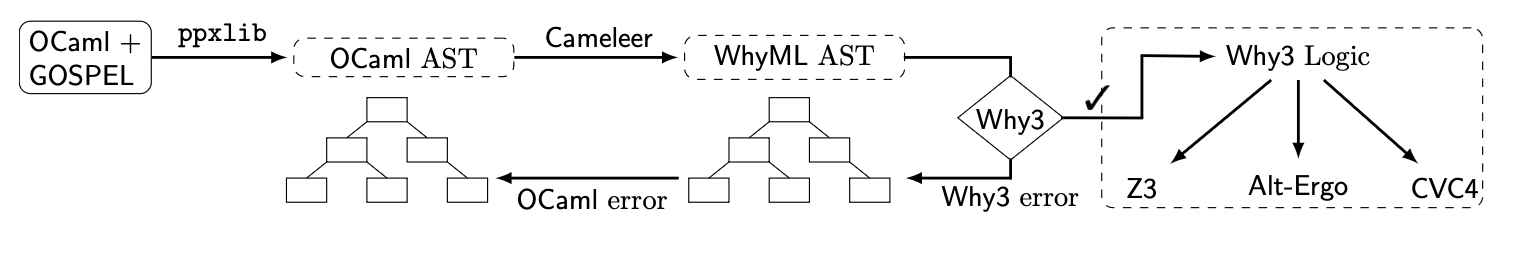
\includegraphics[width=\linewidth]{images/Cameleer_From_Paper.png}
    \caption{The Original Cameleer Pipeline~\cite{PereiraR20}}
    \label{fig:CameleerPipeline}
\end{figure}

In figure \ref{fig:CameleerPipeline} demonstrates how the translation mechanism integrates with surrounding frameworks to produce 
deductively verified \ocaml code annotated with \gospel specifications. If an error is detected in the original \ocaml code during 
translation, the process reverts to the source, requiring corrections to ensure that the generated \whyml code is syntactically and 
semantically valid. Within the \whythree tool, if the generated verification goals cannot be discharged by the automated provers, it indicates 
that the specifications may be imprecise or incomplete and require refinement. These issues are highlighted by the tool, guiding the 
user to improve the annotations. Once all verification conditions are successfully proven, the resulting program is guaranteed to 
be free from compiler-introduced bugs or errors, ensuring a high level of formal correctness~\cite{Filliatre11}.

It is important to distinguish two broad methodologies in deductive verification. On one hand, extraction-based verification involves 
developing verified programs directly within a proof assistant and then extracting executable code, ensuring correctness by construction. 
On the other hand, translation-based verification starts from existing codebases, often annotated with formal specifications, and translates 
them into an intermediate verification language. Verification conditions are then generated and discharged by automated or interactive 
theorem provers. The \cameleer pipeline in figure \ref{fig:CameleerPipeline} follows the translation-based paradigm, 
leveraging \whyml as the intermediate language for verification~\cite{Leroy09}.

\subsection{Cameleer Example}
\label{subsec:CameleerExample}

Let us take this simple example for a recursive factorial in \ocaml + \gospel after applying the \cameleer tool:

\begin{gospell}
let rec fact_aux n c t =
  if c <= n then fact_aux n (c+1) (t*c) else t
(*@
  r = fact_aux n c t
  requires n >= 0
  requires 0 < c <= n+1
  requires t = factorial (c-1)
  ensures r = factorial n
  variant n+1-c
*)
\end{gospell}

The auxiliary function \inlinecode{fact\_aux} receives as arguments the \inlinecode{n} value, that represents the factorial we want to 
compute, the \inlinecode{c} value, that represents the current index of the iteration, and \inlinecode{t} value, that is accumulating 
the result from previous iterations, in order to display the solution.

The specifications include a few pre-conditions, from those, the factorial to compute is higher or equal to 0, because the factorial as 
default is only calculated for non-negative values, the index of the iteration is between 0 and factorial to compute, because from the
code written when the index achieves the same value as the factorial to compute the function should terminate. For the post-conditions
we only need to make sure the result of the auxiliary function is indeed the factorial of n, which is calculated logically with the 
definition below. The variant serves to prove the termination of the recursive function with an expression that decreases every iteration
and is limited by 0. In this case since the counter is approaching n+1 every iteration, for the last iteration t holds the factorial of n,
which was the previous value of c and terminates successfully.

In the specification of function \inlinecode{fact\_aux} we use the logical definition of the factorial function which we present below:

\begin{gospell}
(*@ 
  function rec factorial (n:int) :int = 
    if n=0 then 1 else n * factorial (n-1)
*)
(*@ 
  requires n >= 0
  variant n
*)
\end{gospell}

This \gospel function represents the logical concept of a factorial, this can be used in other specifications 
to compare results. The implementation of this function is in a recursive way, since \gospel only supports the functional paradigm.
Additionally, logical definitions are meant to be simple rather than complex but optimized, since we want to simplify the proof.

Finally, the main function \inlinecode{fact}:

\begin{gospell}
let fact n = fact_aux n 1 1
(*@ 
  r = fact n
  requires n >= 0 
  ensures r = factorial n
*)
\end{gospell}

Initializes the auxiliary call with appropriate base values, the first one is the counter so it needs to start at 1 because for the 
multiplication with the accumulator starting at 0 would not take into consideration the first iteration. For the 1 in the accumulator, 
the third argument, represents the neutral element for multiplication. The \gospel annotations specify the expected behaviour, including 
pre-conditions such as non-negativity of \inlinecode{n} and the correctness of the returned result.

The translated code to \whyml creates 2 goals, one for the function \inlinecode{fact} and another for the logical function
\inlinecode{factorial}. After splitting the goals we get for \inlinecode{fact} the variant and pre-condition, and for
\inlinecode{factorial} the invariant initialization, the invariant preservation, the post-condition and the VC:

\begin{figure}[H]
    \centering
    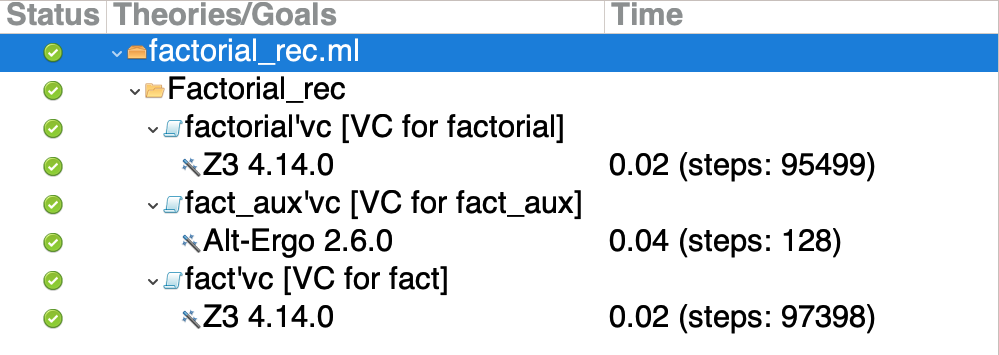
\includegraphics[width=0.7\linewidth]{images/Why3Goals.png}
    \caption{The Goals Proved in \whythree}
    \label{fig:Why3Goals}
\end{figure}

All verification goals were successfully discharged in figure \ref{fig:Why3Goals} through the automated provers, resulting in the 
original \ocaml code, annotated 
with \gospel specifications, being fully verified. This outcome demonstrates the effectiveness of the verification pipeline, 
where the combination of \cameleer and \whythree enables high levels of automation in proving the functional correctness of 
\ocaml programs.